\section{Execution Flow}
\label{design:flow}

Until now we have established how the bootware can be called from outside components using a web service interface and a context to start the bootstrapping process.
We also established that big parts of this process will be implemented as plugins.
Now it is time to take a look at the actual internal structure of the bootware.
What follows is a step by step description of the whole bootstrapping process.

\begin{figure}[!htbp]
	\centering
	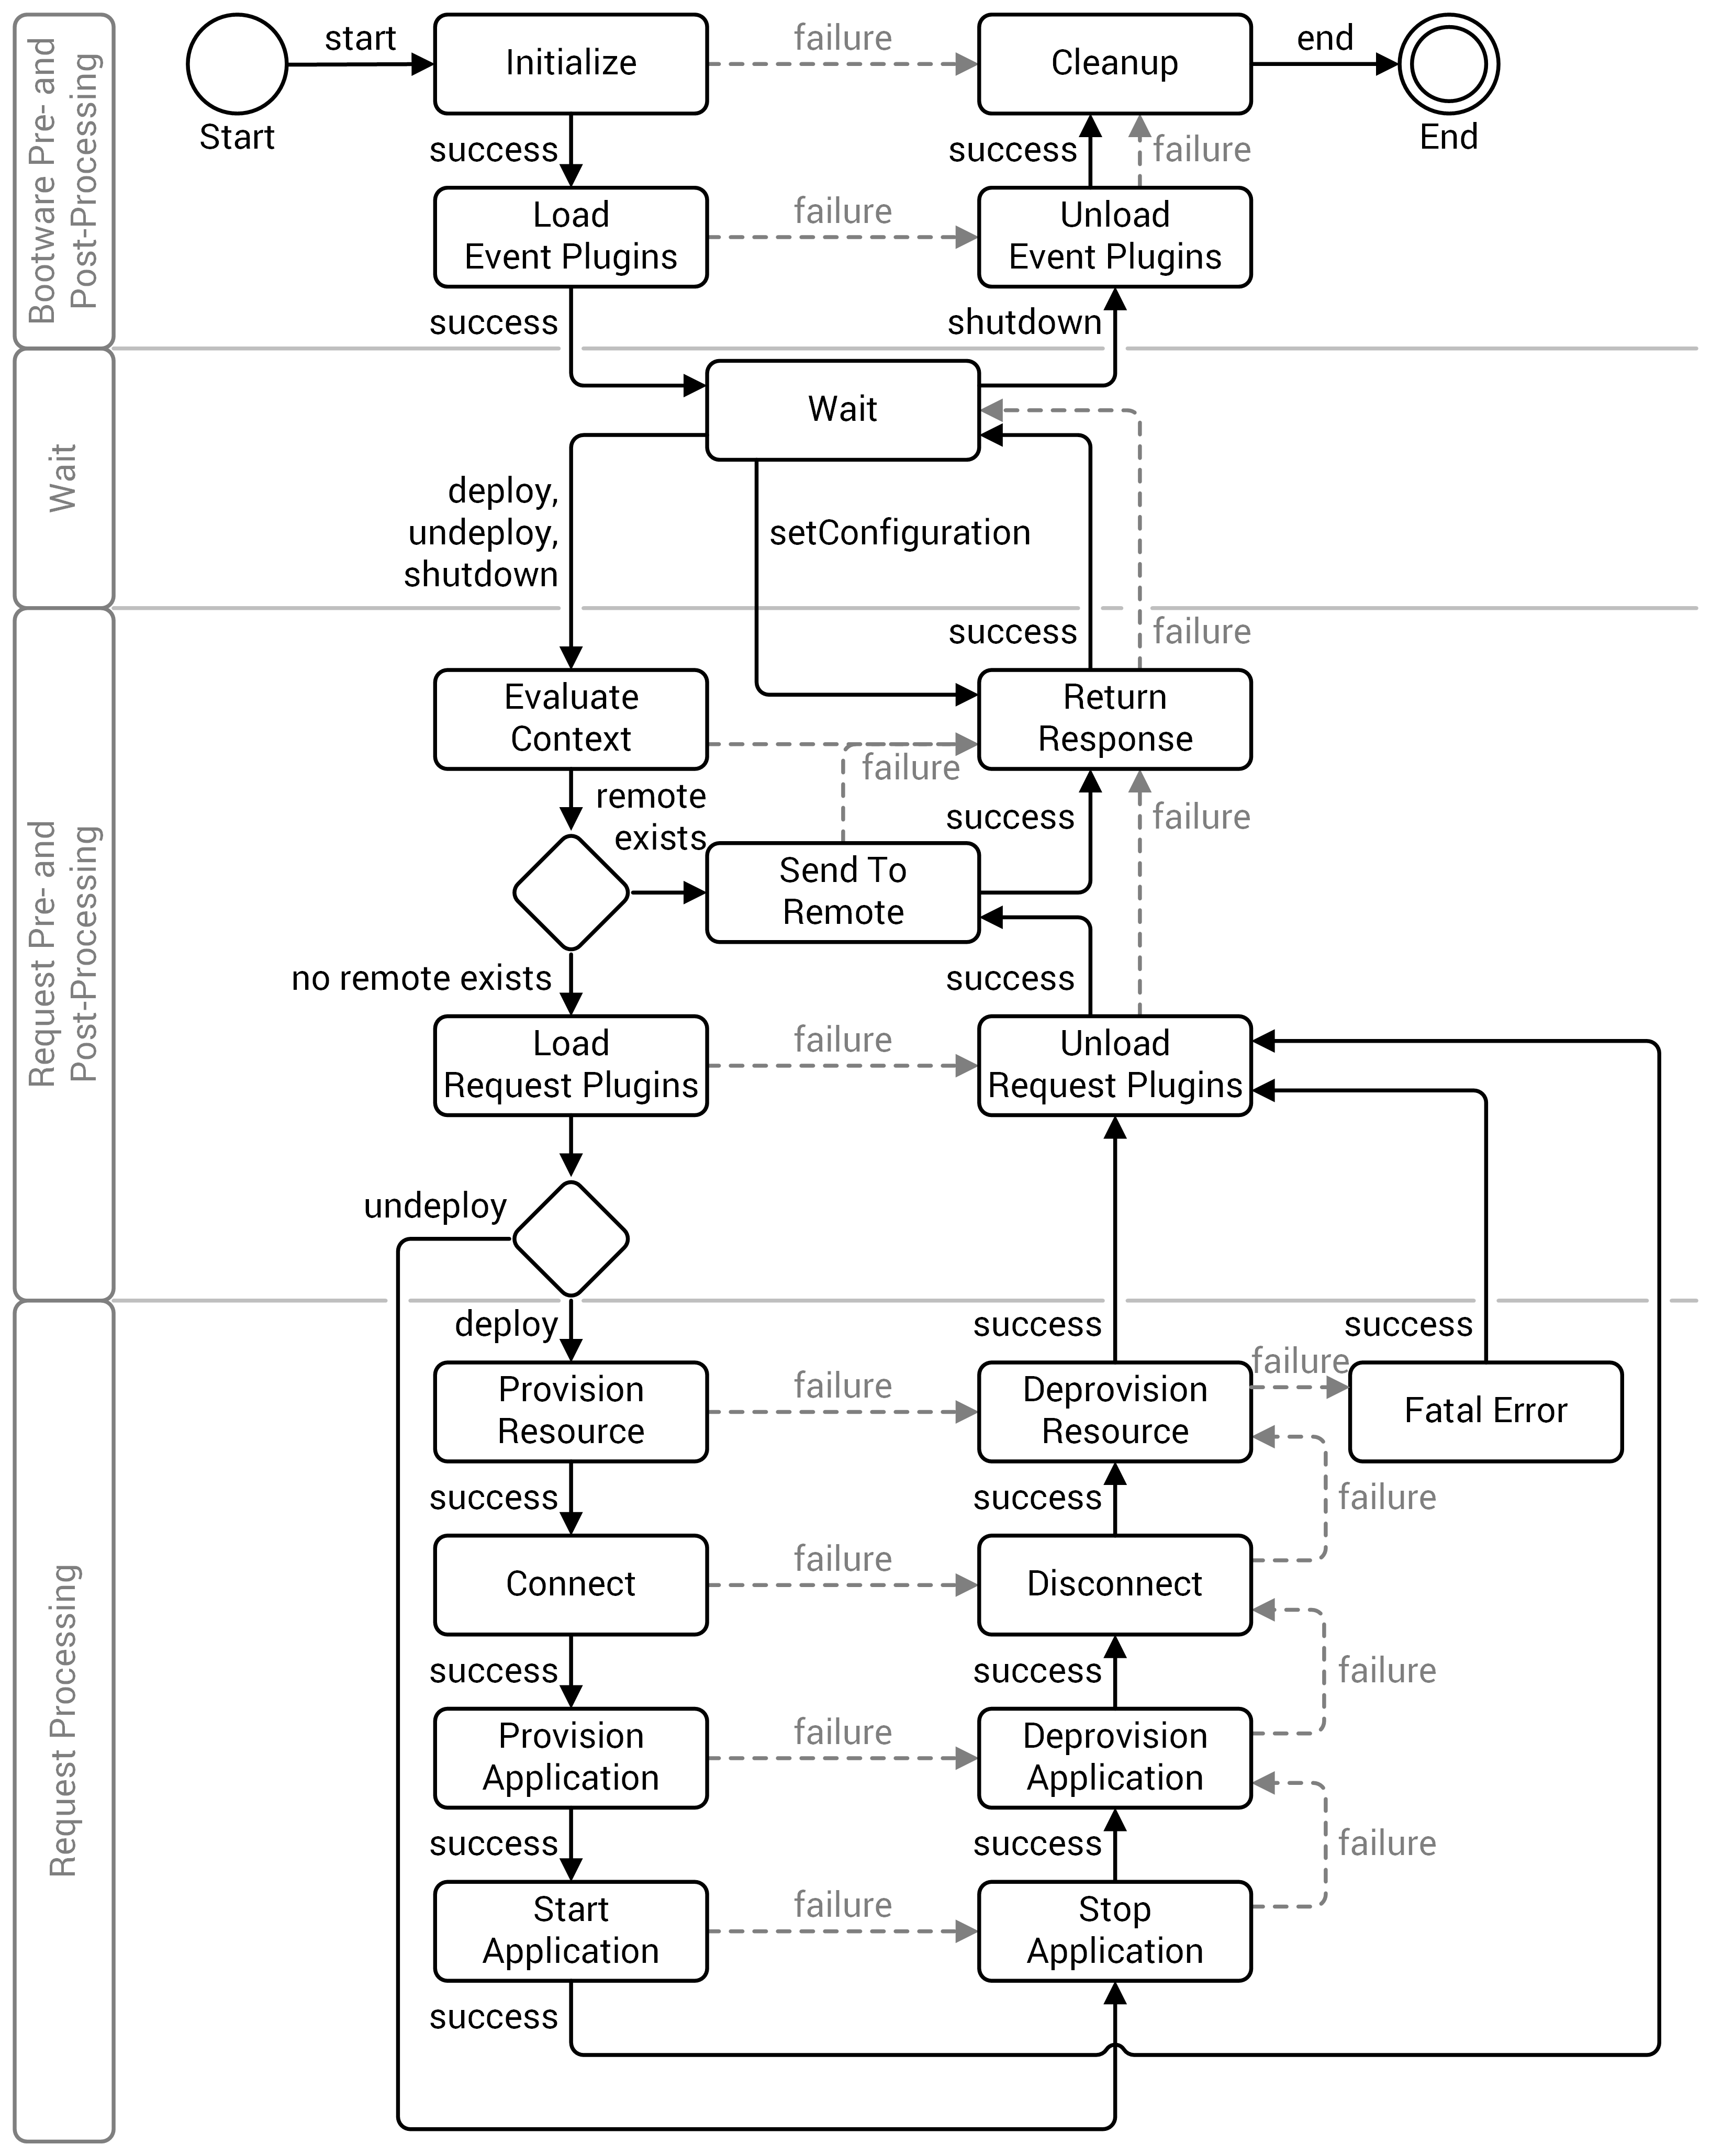
\includegraphics[resolution=600]{design/assets/flow_local}
	\caption{Execution flow in the local bootware.}
	\label{image:flow_local}
\end{figure}

\autoref{image:flow_local} shows a graph that represents the major steps during the bootware execution in the local bootware as flow diagram.
The bootstrapping process is started by executing the local bootware, which is represented by the start state in the top left corner of \autoref{image:flow_local}.
From there, the bootware first does some initializations.
If those fail for some reason, the cleanup code will be executed before the local bootware execution is ended, as can be seen on the top right corner of \autoref{image:flow_local}.
In most cases however, the initialization should succeed.
Then, the local bootware will transition to the next state, where it tries to load the event plugins.

The event plugins are loaded once at the beginning of the local bootware execution because they will not change at a per request basis (like the other plugins).
If loading one of these plugins fails, the local bootware will try to unload already loaded plugins before continuing to the cleanup state.
If the plugins are loaded successfully, the local bootware transitions into the wait state, shown in the top center of \autoref{image:flow_local}.

Once the local bootware is in the wait state it is ready to receive requests from the outside.
If a shutdown event is received in this state, the local bootware will first tell the remote bootware to undeploy all active payloads.
Next, the local bootware will undeploy the remote bootware by running through the undeploy process shown on the bottom left with the appropriate plugins.
Then, it will shut itself down by first unloading the event plugins and then running the cleanup code.
This is the only normal way to shut down the local bootware.
We only hint at the setConfiguration request here because it is so simple that it could also be handled in the wait state.
Deploy and undeploy requests however are more complicated.
If such a request is received in the wait state, the local bootware transitions to the next state, where it reads the request context.

The request context contains all the information necessary to fulfill the request, as described in \autoref{design:context}.
If the context can not be read, the local bootware returns a response containing an error message before returning into the wait state.
If the context is read successfully the local bootware tries to send the request on to the remote bootware, as shown in the middle of \autoref{image:flow_local}.
For this to work, the remote bootware has to exist in the requested remote environment, which will not be the case during the first execution.
Therefore, the local bootware first has to provision the remote bootware in the requested remote environment and so it transitions to the load request plugins state.

In the load request plugins state the plugins specified in the context are loaded.
If this fails, the local bootware tries to unload already loaded plugins before returning an error response and transitioning to the wait state.
If the plugins are loaded successfully, the local bootware now starts either the deploy process or the undeploy process, shown at the bottom of \autoref{image:flow_local}, depending on the type of the request.

If the request was a deploy request, the local bootware will now execute the steps shown in the bottom left of \autoref{image:flow_local} one after another, which include the deploy, connect, and start operations of the infrastructure, connection, and payload plugins.
If one of those operations fails the local bootware transitions over to the corresponding undeploy operation and works its way backwards to undo all operations that where already executed.
This process is the same as the undeploy process, shown on the bottom right of \autoref{image:flow_local}, which is triggered by an undeploy request.

If the stop payload, deprovision payload, or disconnect states fail, the local bootware just continues with the next undeploy state because these operations are not considered critical.
However, if the deprovision infrastructure state fails, the local bootware transitions to a fatal error state, show at the right of \autoref{image:flow_local}, because this step is considered critical.
This state failing could mean that resources are still active in the cloud and human interaction is necessary to remove them to stop further costs from incurring.
The fatal error state is responsible for taking special actions to remedy this situation.

The successful, as well as the unsuccessful execution of either the deploy or the undeploy process all finish in the unload request plugin state, where the plugins that where needed for this particular request are unloaded.
If everything went as planned, a remote bootware should now be running in the desired cloud environment and the local bootware can now pass on the request to this remote bootware, as shown in the center of \autoref{image:flow_local}.
The local bootware will wait in this state until it receives a response from the remote bootware.

Now, we move our attention to the remote bootware, where the requests continues to be processed.
\autoref{image:flow_remote} shows the execution flow of the remote bootware.
As we can see, it is largely identical to the local bootware, at least at the moment.
The send to remote state is gone because it is not needed in the remote bootware.
Instead, as the bottom of \autoref{image:flow_remote} shows, the provision and deprovision middleware steps were added.
The remote bootware also supports the getActivePayloads request.
Other than that, the local and remote processes are the same.

\begin{figure}[!htbp]
	\centering
	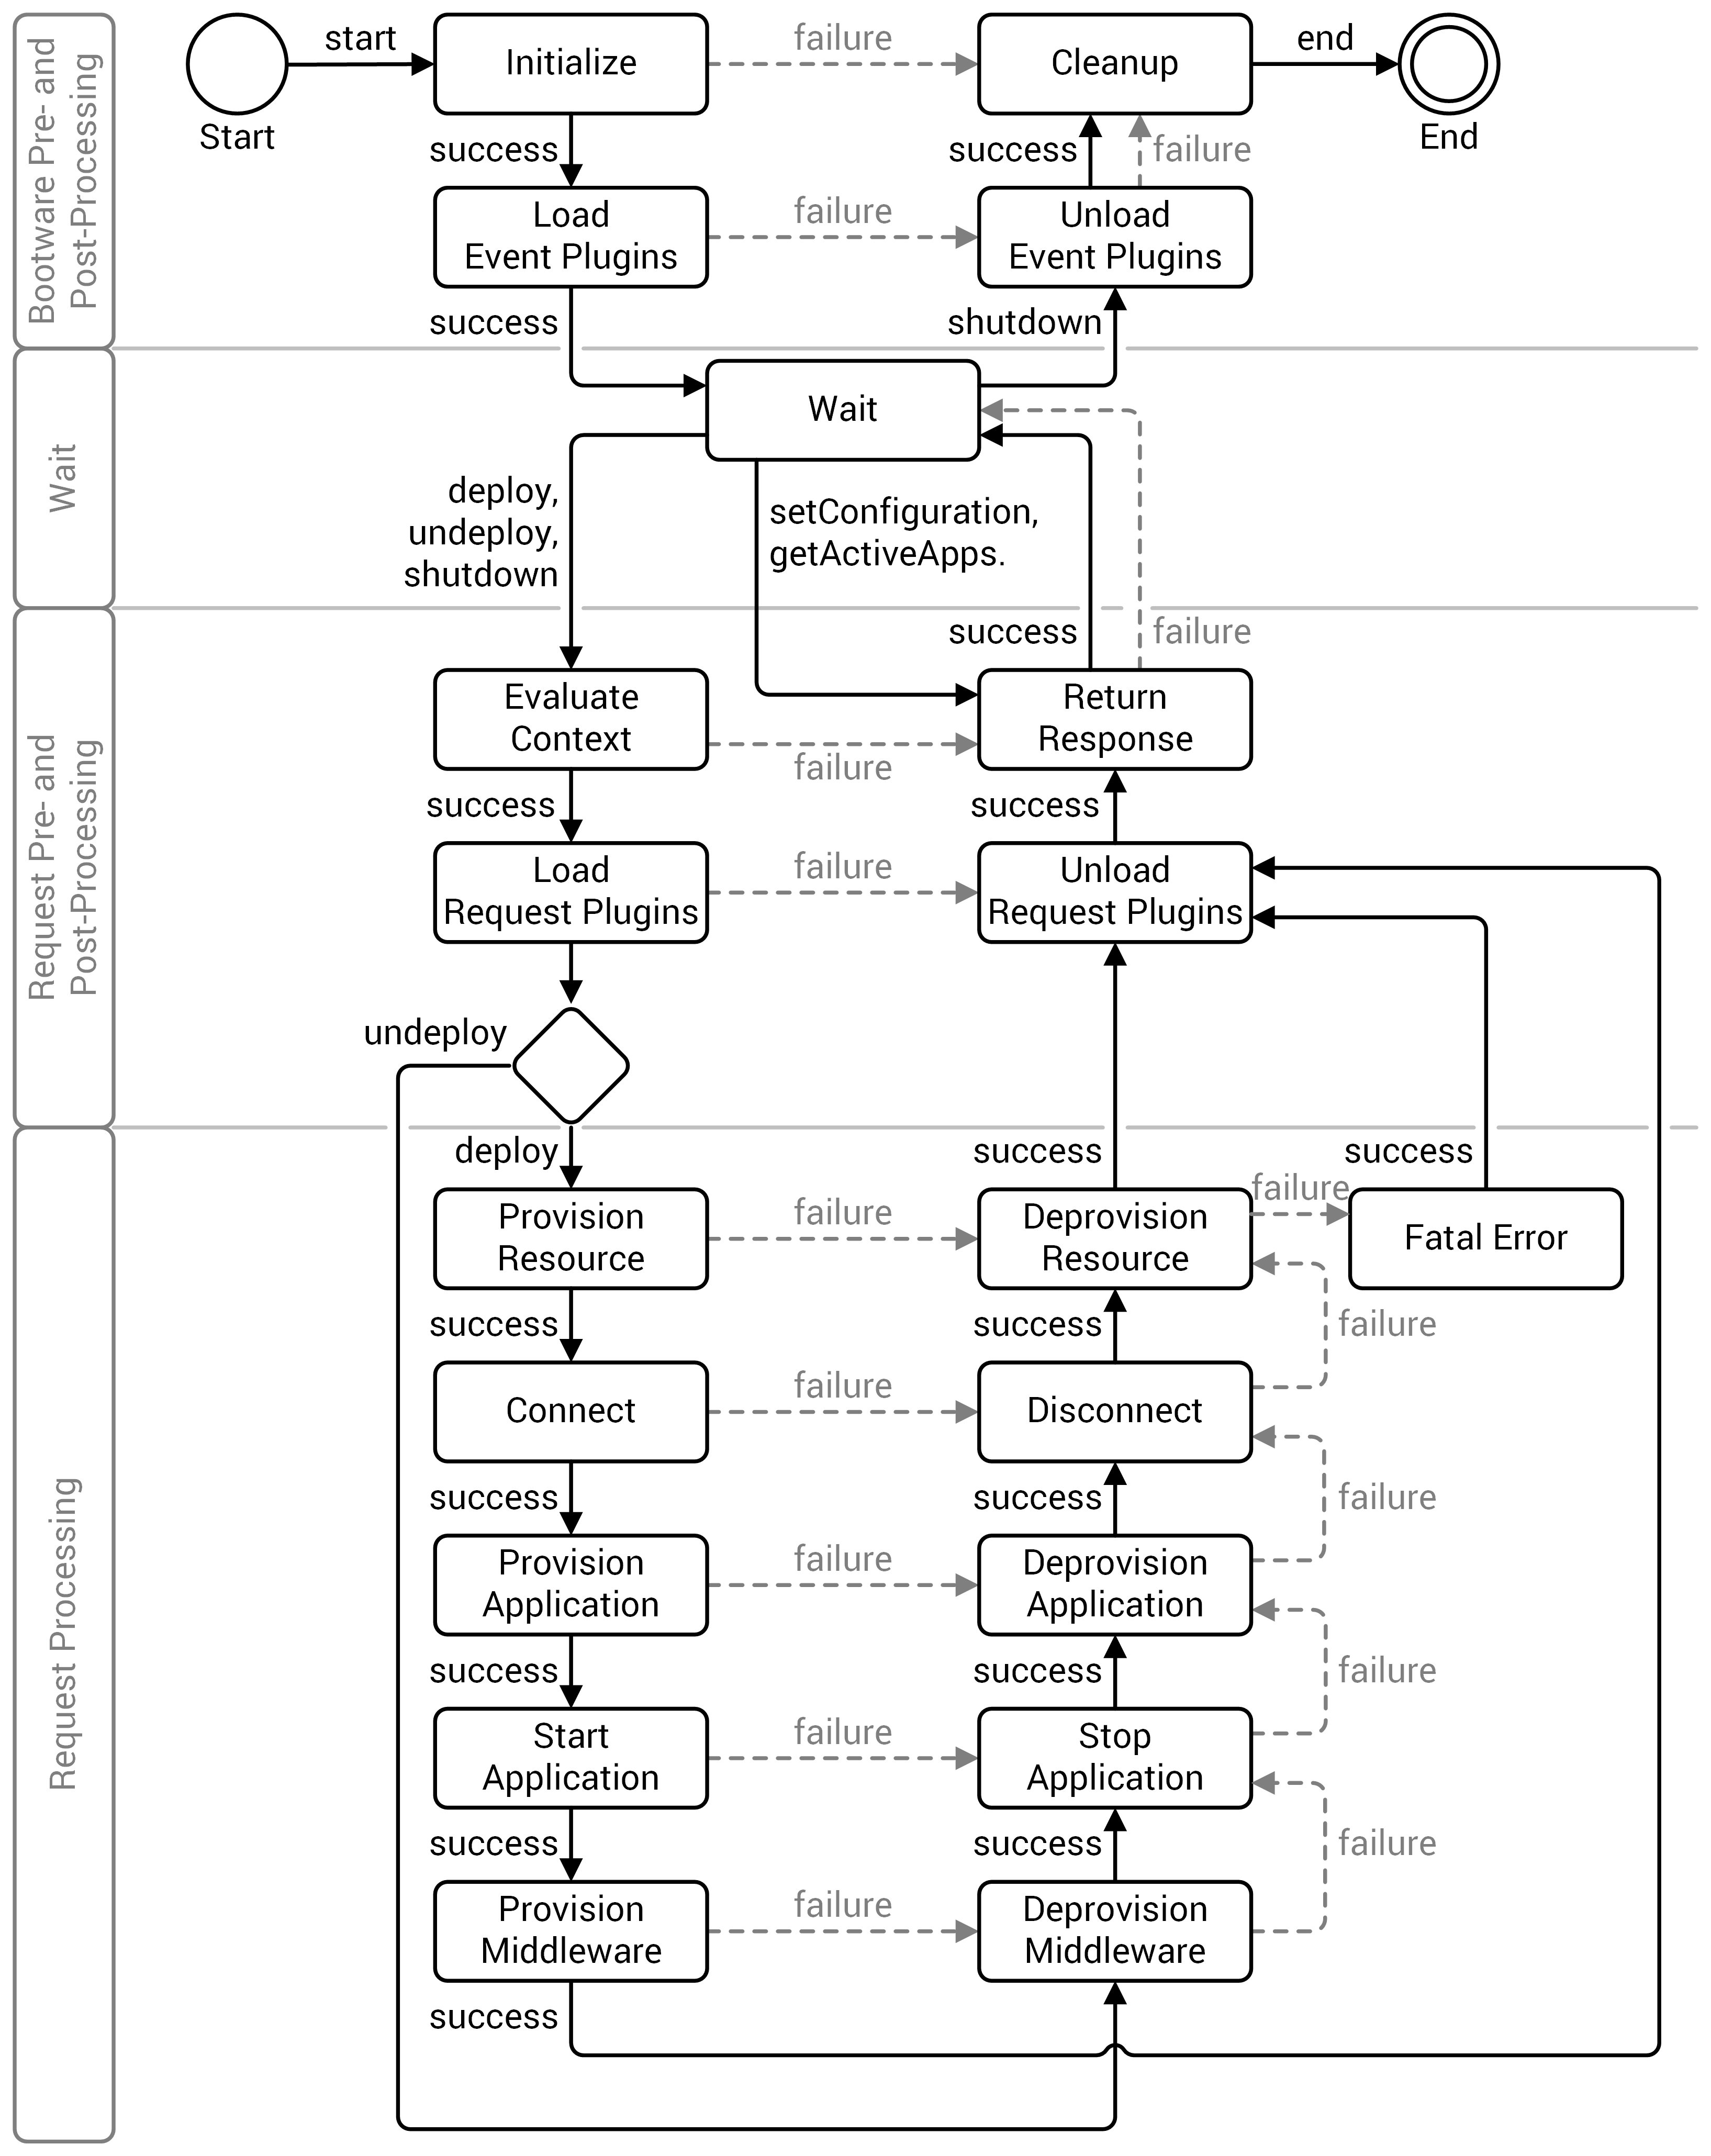
\includegraphics[resolution=600]{design/assets/flow_remote}
	\caption{Execution flow in the remote bootware.}
	\label{image:flow_remote}
\end{figure}

Like the local bootware, the remote bootware went through the initialization steps shown at the top of \autoref{image:flow_remote} when it was started by the local bootware.
It then waited in the wait state for a request.
Now, it receives the request from the local bootware, reads the context, loads the request plugins and executes the deploy operation.
This should result in a provisioning engine being started by the payload plugin.
After that, the remote bootware enters the new provision middleware state at the bottom left of \autoref{image:flow_remote}, which will use the just started provisioning engine to deploy the workflow middleware by executing the call provisioning engine plugin.
Once the middleware is running, the remote bootware is finished with this request and returns the endpoint references of the middleware in the response to the local bootware, before returning into the wait state.

This brings us back to \autoref{image:flow_local}, where the local bootware has now received the answer from the remote bootware in the send to remote state.
Now, the local bootware can finish its request by sending back a response to the bootware adapter, before returning to the wait state.
The local bootware is now done until it is time to undeploy the remote bootware.
Meanwhile, the bootware adapter starts the workflow execution on the middleware, during which multiple calls from the provisioning manager to the remote bootware will occur, which will each time trigger the deploy or undeploy process shown at the bottom, or the getActivePayloads operation only hinted at in \autoref{image:flow_remote}.

As \autoref{image:flow_local}, \autoref{image:flow_remote} and the description above show, this is quite a complicated process with many conditional transition.
Using traditional programming methods like if/else blocks to implement this process would lead to a rather unwieldy and complicated construct with lots of nested if/else block.
Therefore, it could be advantageous to use other methods that are more fitting for this process.
Since we already described the process as a directed graph with states and transition, it would be ideal if we could take this whole graph and use it in the bootware.
Fortunately, this is possible by implementing the process using a finite state machine.

\subsection{Finite State Machine}

In theoretical computer science, a \nom{Finite State Machine}{FSM} is a formal, abstract model of computation that "consisting of a set of states, a start state, an input alphabet, and a transition function that maps input symbols and current states to a next state. Computation begins in the start state with an input string. It changes to new states depending on the transition function"~\autocite{fsm}.
In this context, a state is the "condition of a finite state machine [...] at a certain time. Informally, the content of memory"~\autocite{state}.
The start state is therefore the initial condition of a FSM.
The alphabet is a "set of all possible symbols in an application. For instance, input characters used by a finite state machine, letters making up strings in a language, or symbols in a pattern element. In some cases, an alphabet may be infinite"~\autocite{alphabet}.
The transition function is a "function of the current state and input giving the next state of a finite state machine"~\autocite{transitionfn}.
FSMs can further be distinguished in deterministic and non-deterministic FSMs.
A deterministic FSM has at most one transition for each symbol and state, whereas a non-deterministic FSM can have non, one, or more transitions per symbol and state~\autocite{deterministic}.

Aside from its uses in theoretical computer science, FSMs also have practical applications in digital circuits, software applications, or as lexers in programming language compilers.
We are only interested in the use of FSMs for building software, so we can redefine what a FSM means for our case.
We want to use a FSM as an abstract machine that is defined by a finite list of states and some conditions that trigger transitions between those states.
Unlike a traditional FSM, we will not consume symbols from a set alphabet that will trigger state transitions.
We want the state transitions to be triggered by events that we can emit at any time, so we want an event-driven FSM.
The machine is in only one state at a time, its current state.
At the start of the machine execution, it will be in the start state.
From there, it can transition from one state to another when certain events are triggered, until it finally reaches an end state.
When it enters a state, it executes a function associated with this state.
The result of the execution of this function determines to which state the FSM will transition next.
We will talk more about the actual implementation with FSMs in \autoref{implementation}.
